\documentclass[a4paper,12pt]{article}

% Packages
\usepackage{animate}
\usepackage{amsmath}
\usepackage{amssymb}
\usepackage{bibentry}
\usepackage{color}
\usepackage{dirtree}
\usepackage{float}
\usepackage{geometry}
\usepackage{graphicx}
\usepackage{hyphenat}
\usepackage{indentfirst}
\usepackage{listings}
\usepackage{ipsum}
\usepackage{titlesec}
\usepackage{url}
\usepackage{physics}
\usepackage{fontspec}
\usepackage{wrapfig}
\usepackage{subcaption}
\usepackage{float}
\usepackage[normalem]{ulem}
\usepackage[backend=biber, style=apa]{biblatex}
\usepackage[
colorlinks=true,
linkcolor=blue,
urlcolor=cyan,
citecolor=blue,
breaklinks=true,
]{hyperref} % For hyperlinks

\definecolor{dkgreen}{rgb}{0,0.6,0}
\definecolor{gray}{rgb}{0.5,0.5,0.5}
\definecolor{mauve}{rgb}{0.58,0,0.82}
\lstset{
	aboveskip=3mm,
	basicstyle=\ttfamily\small,
	belowskip=3mm,
	breakatwhitespace=true,
	breaklines=true,
	columns=flexible,
	commentstyle=\color{dkgreen},
	frame=none,
	keywordstyle=\color{blue},
	language=C++,
	numbers=none,
	numberstyle=\tiny\color{gray},
	showstringspaces=false,
	stringstyle=\color{mauve},
	tabsize=4
}
\addbibresource{references.bib}
\geometry{margin=1in}
\titleformat{\chapter}[display]
{\normalfont\huge\bfseries}{\chaptertitlename\ \thechapter}{20pt}{\Huge}
\titlespacing{\chapter}{0pt}{0pt}{0pt}
\sloppy

% Title and Author
\title{Computational Fluid Dynamics With a Paper Airplane}
\author{
  Tasada, Daniel\\
  \and
  Tse, Nathan\\
}
\date{\today}

\begin{document}

% Title and abstract
\maketitle

\pagebreak
\begin{abstract}
	In this paper, we investigate the relationship between an airplane's shape
	and its performance. Our results show that \dots
\end{abstract}

% Table of Contents
\pagebreak
\tableofcontents
\pagebreak

% Introduction
\section{Introduction}
This thesis covers the simulation of the aerodynamics of an airplane, using
our own Computational Fluid Dynamics model (CFD).

The goal is to simulate the airflow around an airplane's body. CFD is a
branch of fluid mechanics that uses numerical methods and algorithms to solve
and analyze problems that involve fluid flows. It is used in many fields,
including aerospace engineering, automotive engineering, and meteorology.

The application of CFD to an airplane is important because it allows testing
of a model's aerodynamic performance without building a physical model, or
have to set up a wind tunnel. The practical alternative is much more expensive
and time-consuming.

The final aim is to determine how the shape of an airplane's body affects its
performance. Part of the project is to dynamically generate 3D models of
airplanes, and simulate the airflow around them. The intention is to use
machine learning to optimize the shape of the airplane's body to maximize
performance.

CFD is challenging in the sense that it requires a good understanding of fluid
dynamics, as well as a good understanding of the math involved. CFD is also
very expensive from a computational perspective, so code optimization is important.

The thesis questions are the following:
\begin{itemize}
	\item{How do the different aspects of fluid dynamics work and how do we
		implement it in a computer program?}
	\item{How do we dynamically generate 3D models?}
	\item{How does an airplane's wing shape influence its performance?}
\end{itemize}
\pagebreak

\section{Preliminary Research}
In this paper we aim to create our own CFD model. 
Before we start creating our own model a understanding of how CFD models work 
and the different types of models and methods that can be used is needed.
Most CFD models are based on the Navier-Stokes equations. Because the Navier-Stokes equations are very complex we will not be covering them in depth, 
but we will explain what they are and how they are used in CFD models.
This will be covered in section \ref{navierstokes}.
In section \ref{eulerianlagrangian} we will be looking at two different types of methods that are used to simulate fluid dynamics.

\subsection{Navier-Stokes equations} \label{navierstokes}
The base of almost all CFD models are the \href{https://en.wikipedia.org/wiki/Navier%E2%80%93Stokes_equations}{Navier-Stokes equations}.
These are partial differential equations that describe single-phase fluid flows. 
We will not go to much into detail about these equations, but its important to know that by solving these equations we will get a flow velocity.
This flow velocity is a vector field that gives a vector to every point in the fluid at any time. 
Using this velocity field the behavior of the fluid can be simulated.

\subsection{Eulerian vs Lagrangian} \label{eulerianlagrangian}
There are two main methods to simulate fluid dynamics: the Lagrangian method and the Eulerian method. \\

\textbf{Lagrangian} \\

\begin{figure}[H]
	\centering
	\includegraphics[width=10cm]{resources/lagrangian.png}
	\caption{Lagrangian fluid simulation from (\cite{seblague})}
\end{figure}

The Langrangian method models the fluid as a particle collision system, where the air is represented by
particles that follow the flow velocity and interact with each other to emulate a fluid. 
This method is mostly usefull when trying to analyze situations where single fluid particles play an important role.\\


\textbf{Eulerian} \\

\begin{figure}[H]
	\centering
	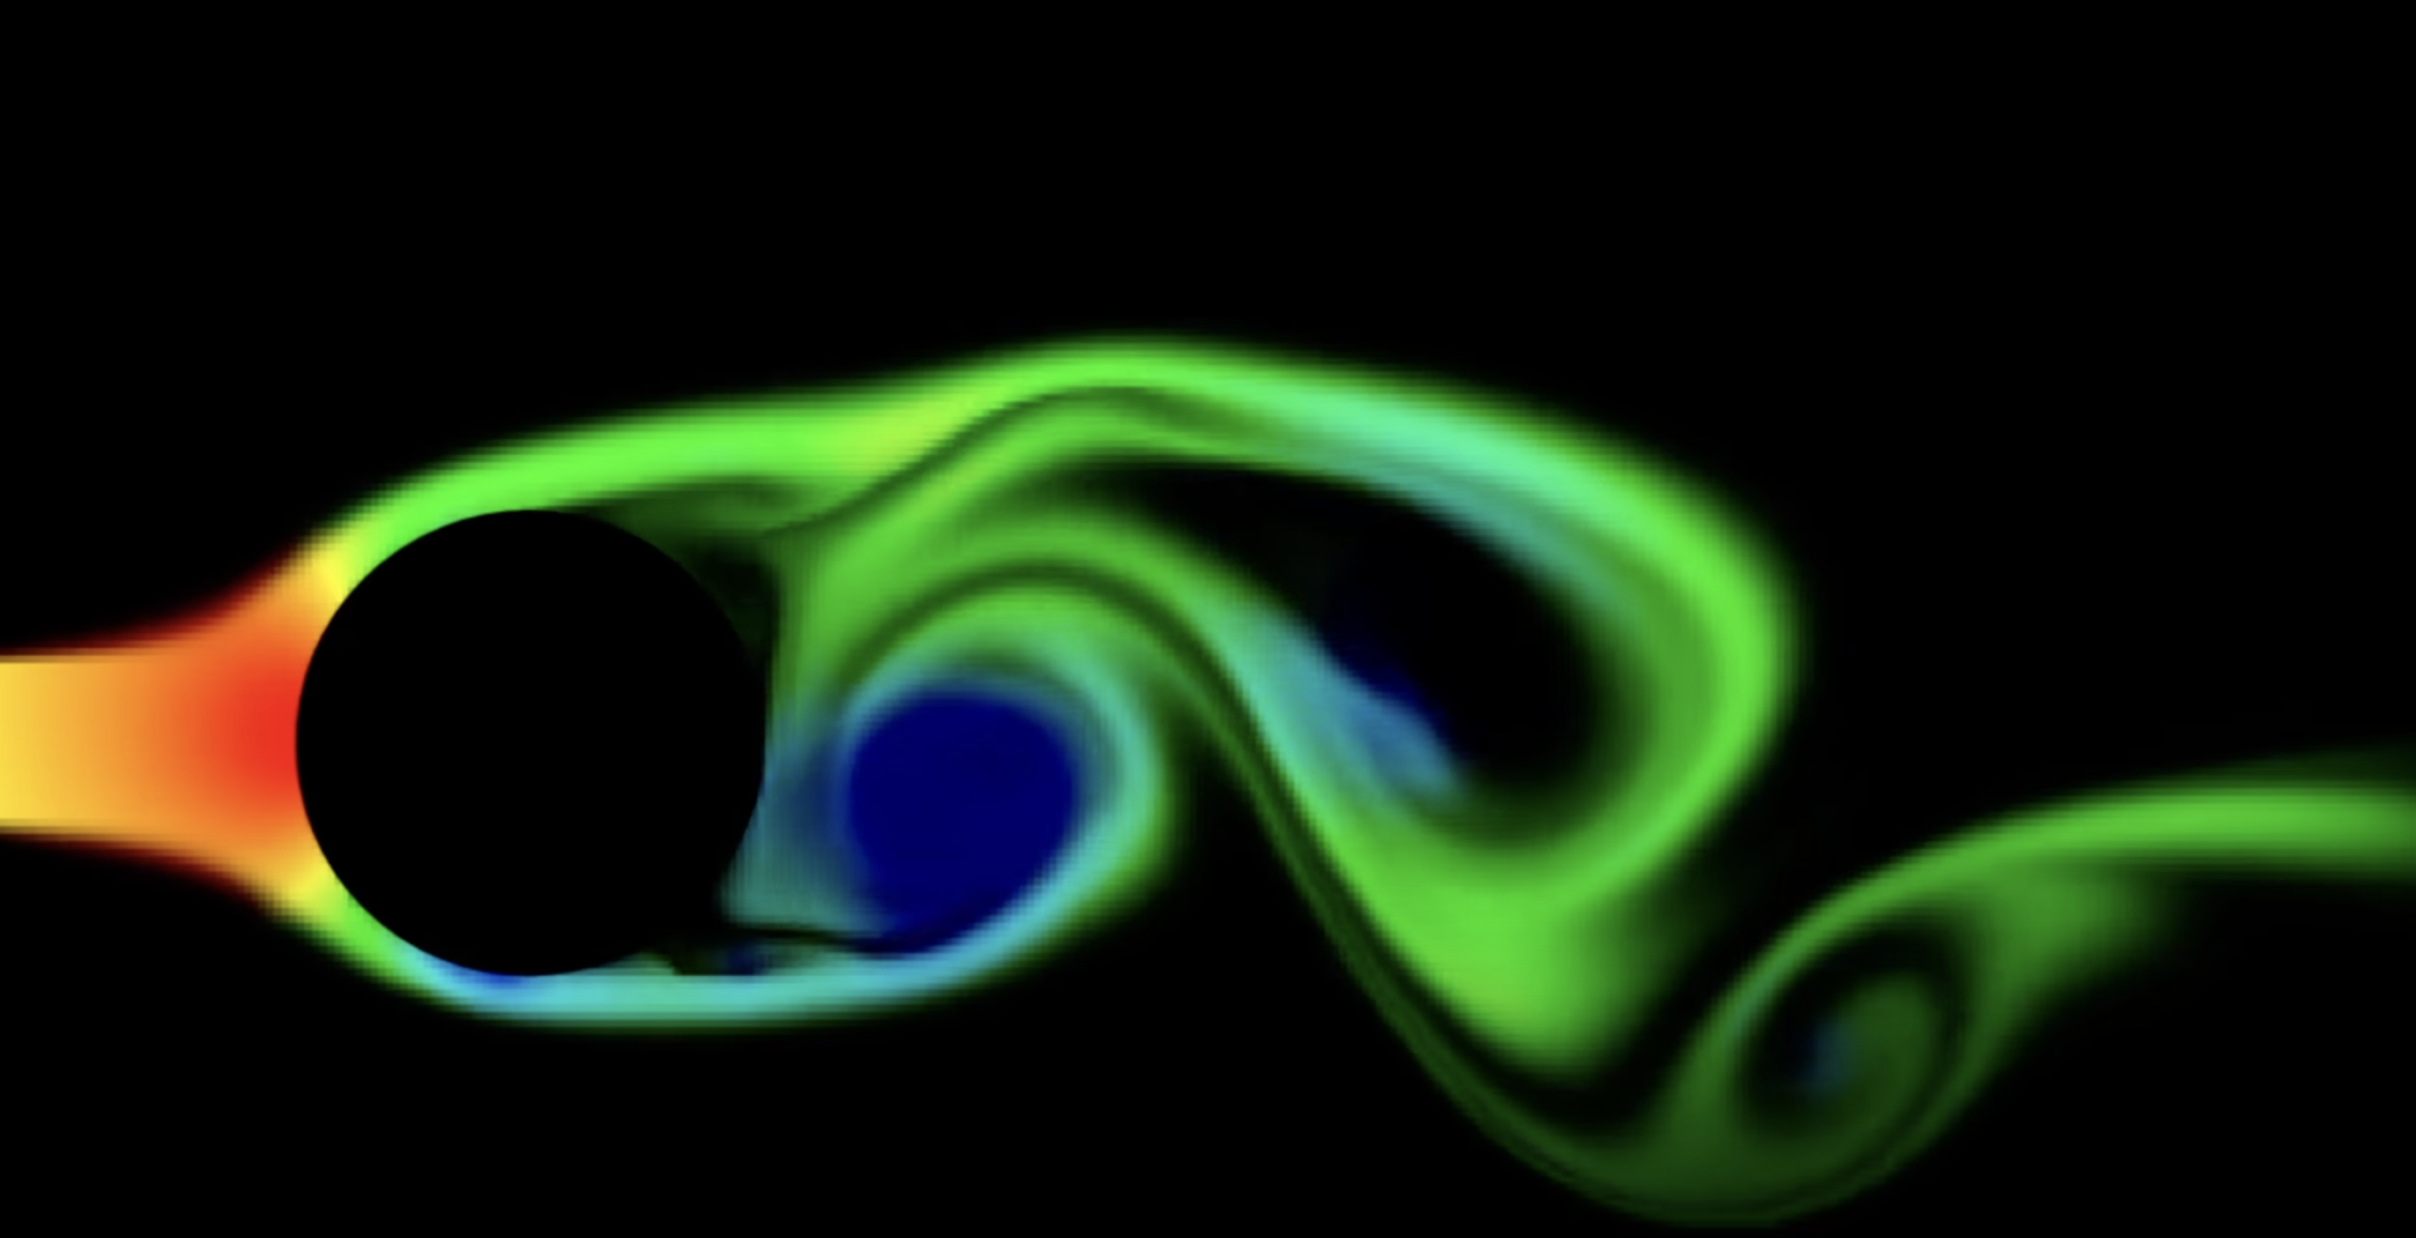
\includegraphics[width=10cm]{resources/eulerian.png}
	\caption{Eulerian fluid simulation from (\cite{tenminute})}
\end{figure}

The other method is the Eulerian method. This method models the fluid as a
cellular automata. The fluid is represented by a grid of cells, each of which
has its own properties and interacts with its neighbor cells, creating a Cartesian
mesh-style field. This method is mostly used when trying to analyze the fluid as a whole.
It can provide information about the fluid's flow patterns, turbulence, and pressure distribution. 

\subsection{NEAT}
NEAT (NeuroEvolution of Augmenting Topologies) is a machine learning algorithm

% Execution
\pagebreak
\section{Preliminary: Lagrangian Fluid Simulation}
We first tried to implement a Lagrangian fluid simulation.
Our implementation is based on \hyperlink{http://www.hakenberg.de/diffgeo/collision_resolution.htm}{Rigid Body Collision Resolution}
(\cite{hakenberg}). We used this paper as a guide for all the math involved.

The math relies on the momentum, inertia, and velocity of the particles to
calculate the collision normal and point of contact. The collision normal is
the direction in which the particles are moving away from each other, and the
point of contact is the point at which the particles collide.

The following variables are necessary to perform the calculations:
\[
\begin{array}{ll}
	\text{Angular momentum $L$ } (kg\cdot m^2/s): & L = mvr; \\
	\text{Inertia tensor $I$ } (kg\cdot m^2): & I = \frac{L}{\omega}; \\
    \text{Angular velocity $\omega$ } (rad/s): & \omega = \frac{\Delta \theta}{\Delta t}; \\

	\\

	\text{Collision normal} (n \in \mathbb{R}^3) \text{ in world coordinates away from body}; \\
	\text{Point of contact } (r_i \in \mathbb{R}^3) \text{ in world coordinates with respect to $p_i$}; \\
	\text{Orientation } (R_i \in SO(3)) \text{ transforming from object to world coordinates}; \\
\end{array}
\]

Where $i$ represents one of two particles in a given collision:
\[
\begin{array}{ll}
	\text{Velocity after collision} & \tilde{v}_i, \\ 
	\text{Angular velocity after collision} & \tilde{\omega}_i, \\
	\text{Constant} & \lambda, \\
\end{array}
\]

The following formulas represent the relation between particles:
\[
\begin{array}{cc}
	\tilde{v}_1 = v_1 - \frac{\lambda}{m_1} n; \\ 
	\tilde{v}_2 = v_2 + \frac{\lambda}{m_2} n; \\
	\tilde{\omega}_1 = \omega_1 - \Delta q_1; \\
	\tilde{\omega}_2 = \omega_2 + \Delta q_2; \\

	\text{where } q_i := I_i^{-1} \cdot R_i^{-1} \cdot (r_i\times n), \\
	\text{and } \lambda = 2 \frac{n v_1 - n v_2 + \omega_1 I_1 q_1 - \omega_2 I_2 q_2}
	{(\frac{1}{m_1} + \frac{1}{m_2})n^2 + q_1 I_1 q_1 + q_2 I_2} \\
\end{array}
\]

This was implemented using Go and raylib, and the code is available at
\href{www.github.com/dtasada/paper}{github.com/dtasada/paper} at the \lstinline{lagrangian-go} branch.

When dealing with a lot of particles, the simulation stops performing as well,
because the number of calculations and iterations of the formulas listed above
has a time complexity of $O(n^2)$, where $n$ is the number of particles. This is
because every particle handles collisions with every other particlee every
single frame. This can be elegantly mitigated by implementing a three-dimensional
grid system, where every particle is assigned to a cell in the grid. This way,
particles only need to check for collisions with other particles in the same cell
or neighboring cells. If the particles are evenly distributed within the container,
each particle only needs to handle collisions with particles in its own cell, and
its 26 neighboring cells. This reduces the time complexity to $O(n)$.

The simulation was unstable at higher densities, where particles would phase
into each other instead of cleanly bouncing. The bug is likely quite simple to
fix, but we got distracted by another method. Despite the optimizations we
made, Lagrangian simulation is still quite computationally expensive, and Go
probably wasn't doing it any favors (Go isn't very memory efficient). In the
end it was put aside, and the Lagrangian implementation was never completed.

\pagebreak
\section{Execution: Eulerian Fluid Simulation}
Our next attempt was to try and implement a Eulerian fluid simulation.
Our fluid simulation involves a three-dimensional grid of cells, each of which
have velocity and density fields. The density fields are purely for the purpose of visualization. When we are talking about 'density',
you can image it as the density of colored dye in the fluid. 
Each frame, the cells interact with each
other according to the \href{https://en.wikipedia.org/wiki/Navier%E2%80%93Stokes_equations}{Navier-Stokes equations}.

The specific math involved in the base equations for the fluid simulation is
quite complex, and we couldn't have derived it on our own, so we used
Mike Ash's implementation \href{www.mikeash.com/pyblog/fluid-simulation-for-dummies.html}{\citefield{mikeash}{title}} (\cite{mikeash})
as the bedrock of our program. Mike Ash's code is in turn based on Jos Stam's
brilliant work on \href{www.dgp.toronto.edu/public_user/stam/reality/Research/pdf/GDC03.pdf}{\citefield{josstam}{title}} (\cite{josstam}).
This math will be explained in section \ref{math}. 
How we implemented this math into the density solver of the fluid simulation is explained in section \ref{density}.
The way it is implemented in the velocity solver is explained in section \ref{velocity}.
We will be explaining the concepts in 2D, so it is easier to visualize and understand. 

% Math
\subsection{The Math} \label{math}
In Eulerian fluid dynamics we represent fluids with a velocity vector field. This means we assign a velocity vector to every point in space.
The Navier-Stokes equations show us how these velocity vectors evolve over time with an infinitely small timestep.
\[
	\begin{array}{ll}
		\pdv{u}{t} = -(u \cdot \nabla)u + v\nabla^2 + f \\
		\\
		\pdv{\rho}{t} = -(u \cdot \nabla)\rho + k\nabla^2\rho + S
	\end{array}
\]
The first equation returns the change in velocity in a vector notation. 
Unlike in Lagrangian fluid simulation, in Eulerian fluid simulation the fluid is not represented by individual particles. 
Thats why, instead, fluid density is used, which tells us the amount of particles present in a point in space. 
The second equation shows us the change of this density. 
Although to understand the math behind this simulation it isn't needed to fully understand these equations, it should be noted that the two equations above look a lot like each other,
as this was helpful in developing the simulation. (\cite{josstam})

\begin{figure}[H]
\centering
\begin{subfigure}{.5\textwidth}
	\centering
	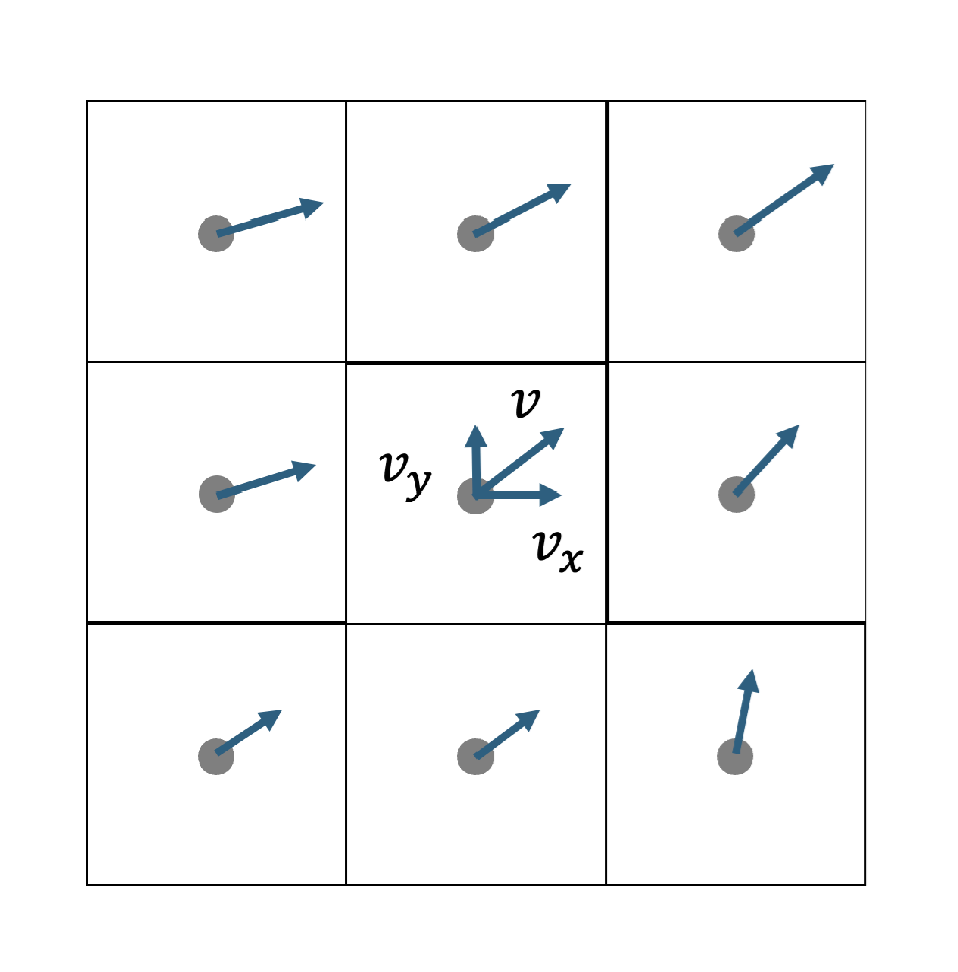
\includegraphics[width=5cm]{resources/collocated_grid_2.png}
	\caption{Collocated grid}
\end{subfigure}%
\begin{subfigure}{.5\textwidth}
	\centering
	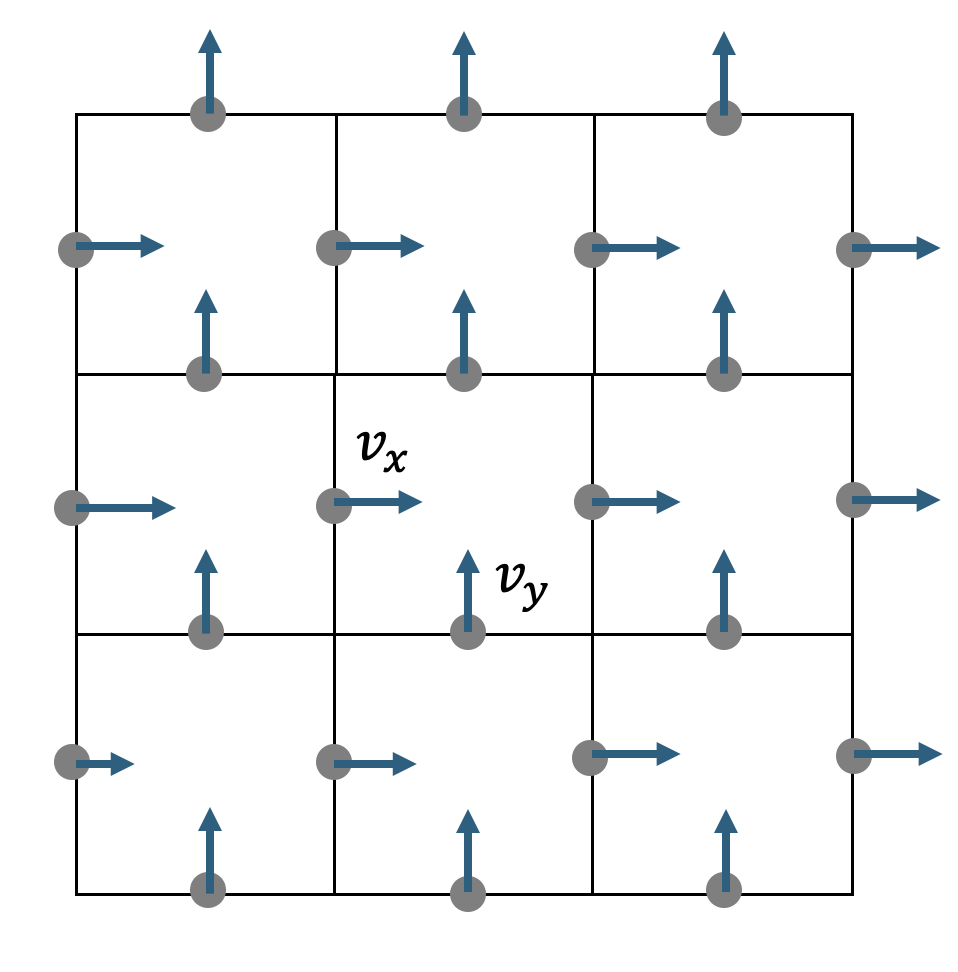
\includegraphics[width=5cm]{resources/staggered_grid_2.png}
	\caption{Staggered grid}
\end{subfigure}
\caption{Computational grids}
\label{fig:grids}
\end{figure}

There are two different types of velocity vector fields we can use: collocated and staggered.
In the collocated grid all the variables are stored in the center of the cell. 
Whereas in the staggered grid the scalar variables are stored at the center but the velocity variable is stored at the cell face. 
Usually the use of a staggered grid is preferred, because its easier to see how much fluid flows from one cell to another. (\cite{tenminute})
However because Mike Ash and Jos Stam used a collocated grid in their works we decided to use the same grid for simpliciy sake.

\subsection{Density Solver} \label{density}

First, lets look at the density solver. The density solver follows three steps: first adding forces, secondly diffusion and lastly moving the densities. 
If we look at the density equation in section \ref{math}, we see that the change in density in a single time steps is influenced by three terms. 
The first term states that the density should follow the velocity field,
the second term represents the density's rate of diffusion
and the third term says that the density can increase due to sources. 
The density solver will apply these terms in reverse order. 
So, as stated before, first the forces are added, then the diffusion is applied and finally the densities are moved.

\subsubsection{Adding forces}
The first step is adding forces from a source. In our case forces will be added if the user clicks on the screen.
If that happens we will simply add a constant amount of density to the intial density. So:
\[
\begin{array}{ll}
  \rho_{t+dt} = \rho_t + S \cdot dt
\end{array}
\]

\subsubsection{Diffusion}
The second step is diffusion.
Diffusion is the process where spread the fluid from high density cells to low density cells.
The diffusion happens at a constant rate that we will call \textit{D}. 
Now we can simply calculate the diffusion rate \textit{a} by multiplying it with the time step:
\[
\begin{array}{ll}
  a = dt \cdot D
\end{array}
\]
If we take a look at a single cell, we'll see that it exchanges densities with its four neighbors.
The total difference of the densities between the cell and its neighbours can be calculated by the following formula,
where $\rho_{x, y}$ is the current density of the cell at position $(x, y)$:
\[
\begin{array}{ll}
	\rho_{x+1, y} + \rho_{x-1, y} + \rho_{x, y+1} + \rho_{x, y-1} - 4 \cdot \rho_{x, y}
\end{array}
\]
By multiplying the difference in densities with the diffusion rate \textit{a} and adding it to the current density, we calculate new density of the cell. 
This can be seen in the following formula, where P$_{x, y}$ is equal to the density of cell at position (x, y) after the time step:
\[
\begin{array}{ll}
	P_{x, y} = \rho_{x, y} + a \cdot (\rho_{x+1, y} + \rho_{x-1, y} + \rho_{x, y+1} + \rho_{x, y-1} - 4 \cdot \rho_{x, y})
\end{array}
\]
But here we run into a problem. If the diffusion rate is big enough the density in a cell might end up becoming negative.
Imagine, for example, a situation wehere the diffusion rate is equal to 1,  the density of a cell is 1 and the densities of its neighbors are all 0. This means that the density of the cell will become -3.
This of course is not possible.
The solution to this problem is to find the density of the cell when being diffused backwards in time. Which results in the following equation:
\[
\begin{array}{ll}
	\rho_{x, y} = P_{x, y} + a \cdot (P_{x+1, y} + P_{x-1, y} + P_{x, y+1} + P_{x, y-1} - 4 \cdot P_{x, y})
\end{array}	
\]
To solve this system of lineair equations for the unknowns P$_{x, y}$ the \href{https://en.wikipedia.org/wiki/Gauss–Seidel_method}{Gauss-Seidel method} is used. 
(\cite{josstam})

\subsubsection{Advection}

\begin{figure}[H]
	\centering
	\begin{subfigure}{0.3\textwidth}
		\centering
		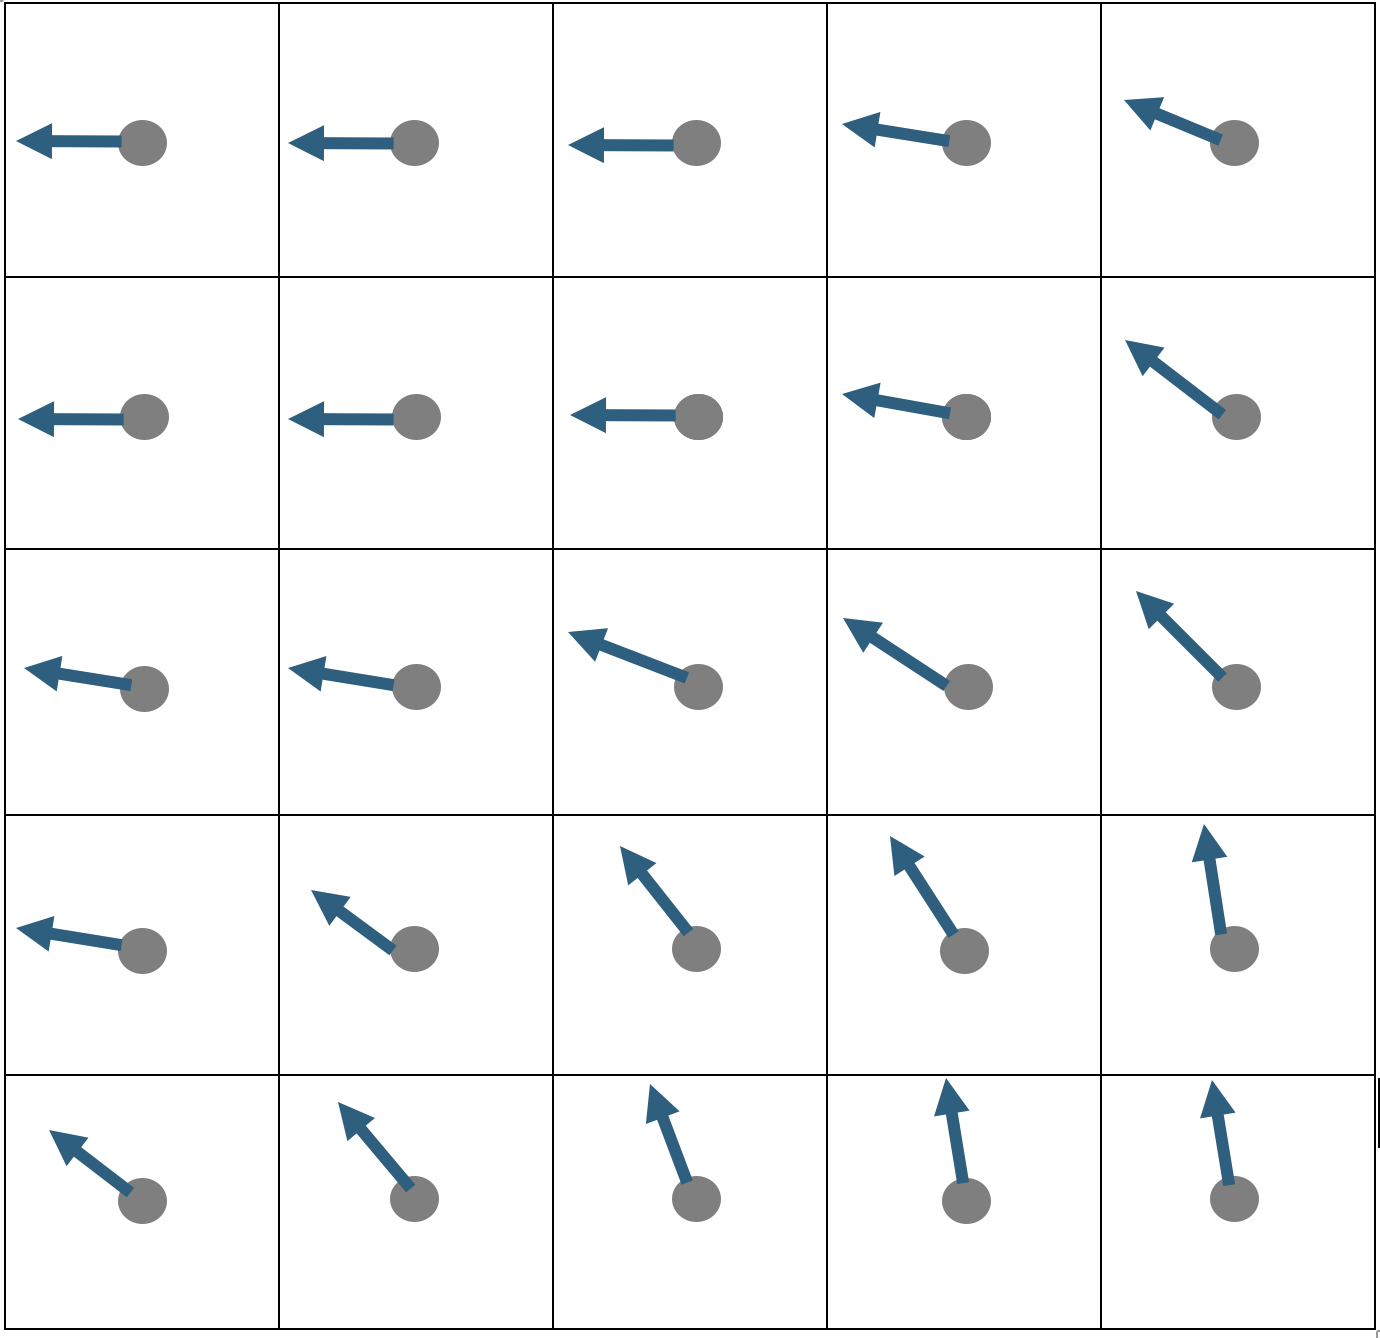
\includegraphics[width=4cm]{resources/advection1.png}
		\caption{Velocity vector field}
	\end{subfigure}%
	\begin{subfigure}{0.3\textwidth}
		\centering
		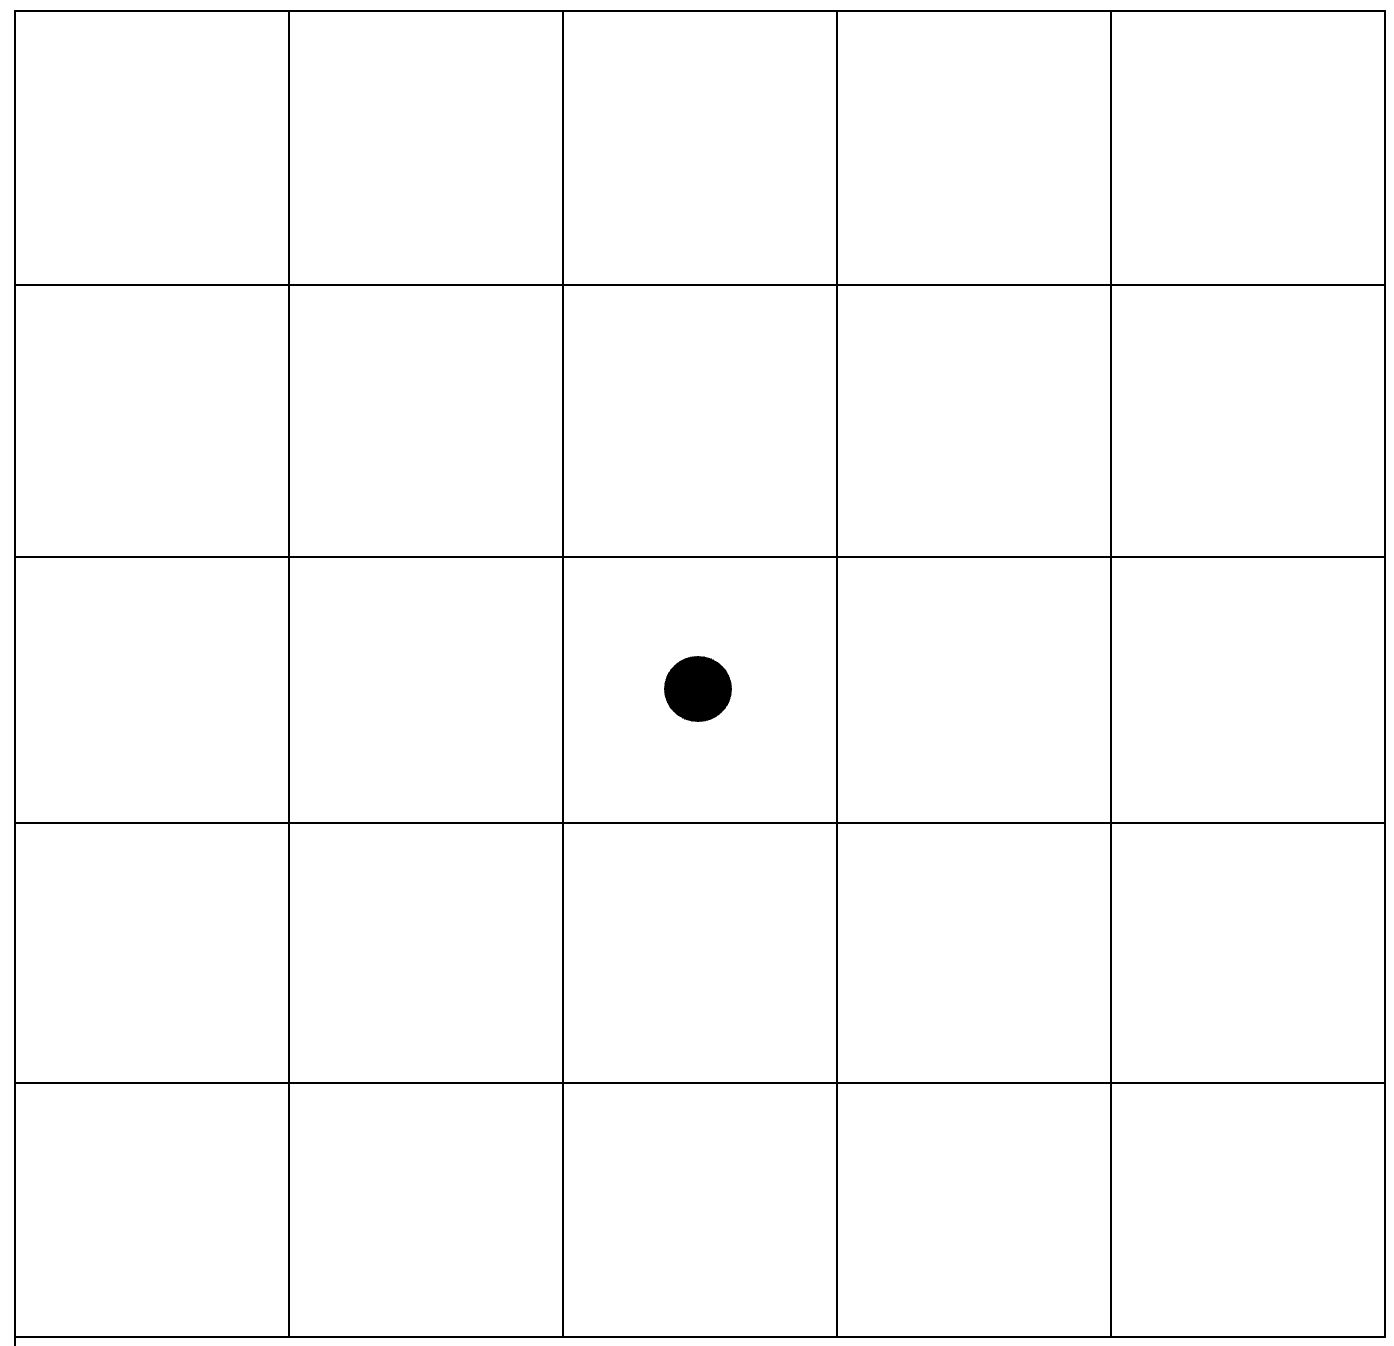
\includegraphics[width=4cm]{resources/advection2.png}
		\caption{A particle}
	\end{subfigure}
	\begin{subfigure}{0.3\textwidth}
		\centering
		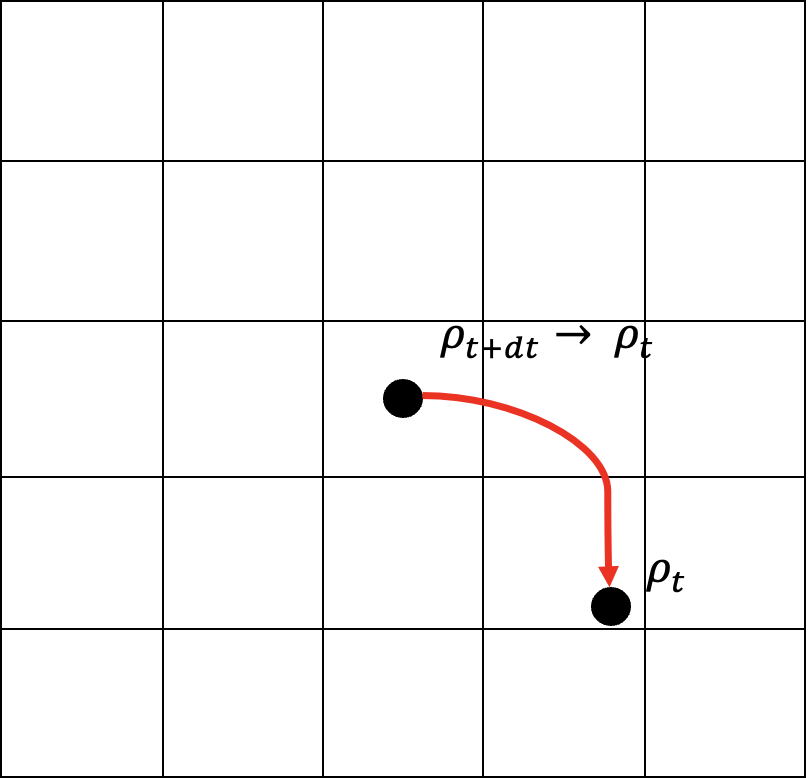
\includegraphics[width=4cm]{resources/advection3.png}
		\caption{Backtracing the particle}
	\end{subfigure}
	\caption {Advection method}
	\label{fig:advection}
\end{figure}

The final step of the density solver is moving the densities following the velocity field.
Because you can't really move grid cells, we will use a technique where we represent a density as a set of particles.
An obvious way to move the densities is to act like the center of a cell is a particle and move it through the velocity field.
But because we have to convert the particles back to a grid, we will use a different method. 
This method is called semi-lagrangian advection.
We will first look at the particles that end up at the center of a cell, as shown in Figure \ref{fig:advection} (b). Then we use the velocity of the cell to trace the particles one time step back in time. This is shown in Figure \ref{fig:advection} (c).
Then we will look at where the particles end up and calculate the weighted average of the densities of the four closest cells from a particle and set this as the new density of the current cell, also shown in Figure \ref{fig:advection} (c).
To do this we need to use two different grids: one that contains all the density values from the previous time step
and on that contains the new density values. (\cite{josstam})
 
\subsection{Velocity Solver} \label{velocity}
Now we will look at the velocity solver. Just like with the density solver if we look at the equations in section \ref{math}
we see that the change in velocity in a single time step is influenced by three factors. 
These are: the addition of forces, viscous diffusion and self-advection. 
Because the velocity equation looks so much like the density equation we can use the same steps that we're shown in section \ref{density} to solve it.
The only difference is that the velocity solver has an extra step called projection.

\subsubsection{Projection}
This step ensures that mass is conserved. 
The law of conservation of mass is an important property of real-life fluids.
The projection step will be the last step that is executed because the previous steps might not always conserve mass.
To make the fluid mass conserving we will use a mathematical concept called Hodge decomposition.
Hodge composition states that every vector field is the sum of a mass conserving field and a gradient field.
So all we have to do is compute a gradient field and subtract it from the velocity field. 
The gradient field 
Computing the gradient field involves the solution of a lineair system called a Poisson equation.
To solve this system we will we again use the Gauss-Seidel method that was also mentioned in section \ref{density} in the diffusion step. (\cite{josstam})

\subsection{The Implementation}
\subsubsection{Introduction to the code}
Our project is structured as follows:
\dirtree{%
	.1 paper.
	.2 neural\DTcomment{Contains ML engine}.
	.2 simulation/\DTcomment{Contains the physics simulation code}. 
	.3 include/\DTcomment{Our own engine headers}.
	.3 resources/\DTcomment{Resources like images, fonts, shaders}.
	.3 src/\DTcomment{Actual engine source}.
	.3 config.toml\DTcomment{Configuration file}.
	.3 Makefile.
}

This codebase is written in C++ and uses \href{https://www.raylib.com/}{raylib} again
because it's a really simple and powerful library that allows us to focus on the
simulation itself, as it provides a bunch of tools to easily render 3D graphics.
The reason this codebase is in C++ was initially because we never got the Eulerian
model to work in Go, likely due to a mistake of our own. Nevertheless we think C++
was the right choice, as it's more appropriate for the vector physics and low overhead
we need for the simulation.

The main fluid simulation object we use for the simulation is the \lstinline{Fluid} class.
The implementation is is available at \lstinline{/simulation/src/Fluid.cpp}.
The interface is as follows:

\begin{figure}[H]
	\centering
	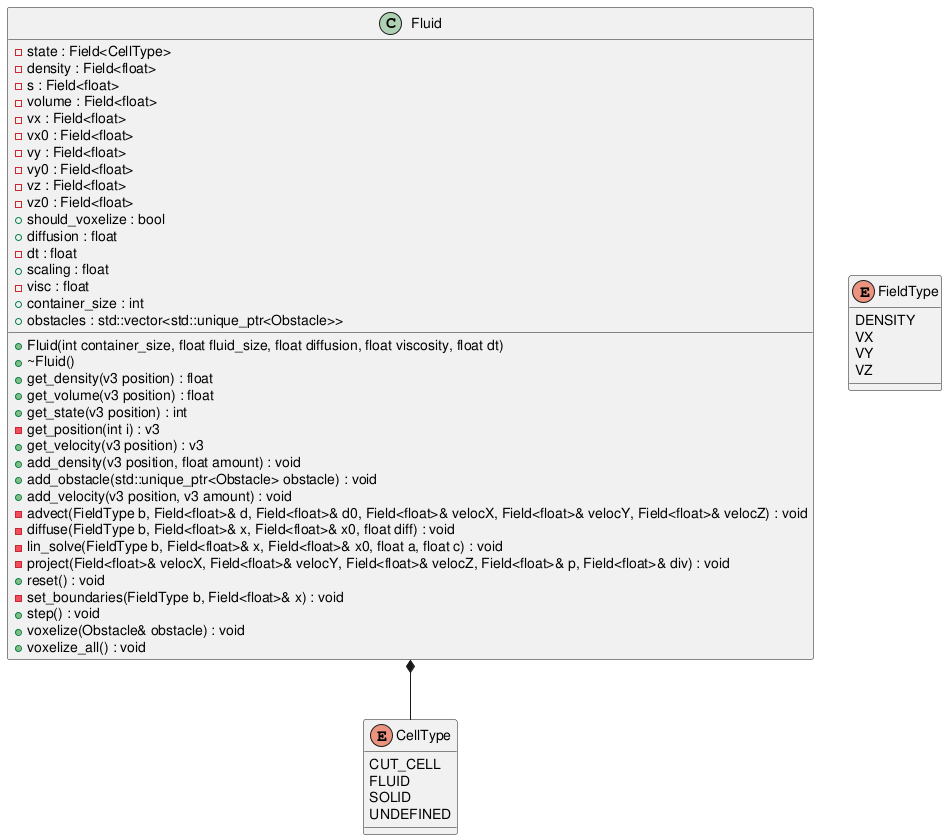
\includegraphics[width=\textwidth]{resources/Fluid.png}
	\caption{Fluid class diagram}
\end{figure}

This class contains the vector fields for the container as well as all the
functions related to the physics simulation, including the advection, diffusion
and projection procedures. These functions are the core of the CFD and
this is the part that we borrowed from Mike Ash.

\begin{figure}[H]
    \centering
    \begin{subfigure}[t]{0.45\textwidth}
        \centering
        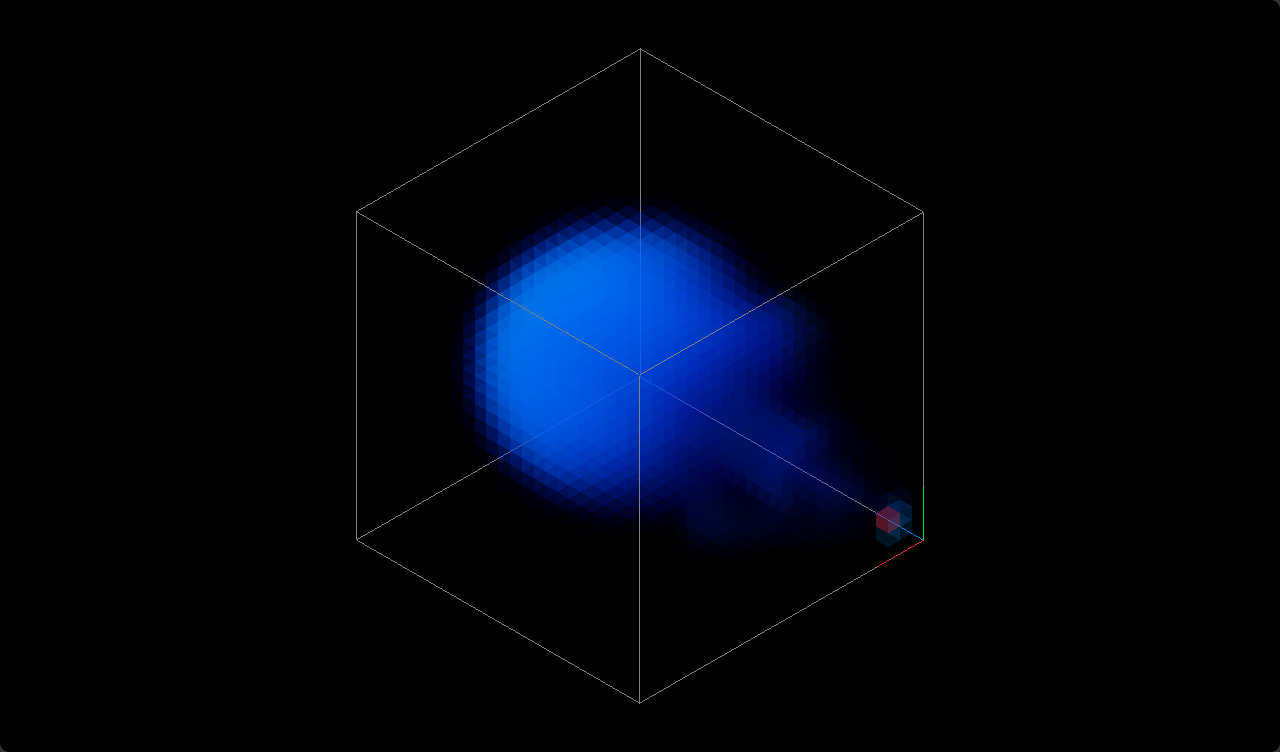
\includegraphics[height=1.65in]{resources/core1.png}
    \end{subfigure}
    \hfill
    \begin{subfigure}[t]{0.45\textwidth}
        \centering
        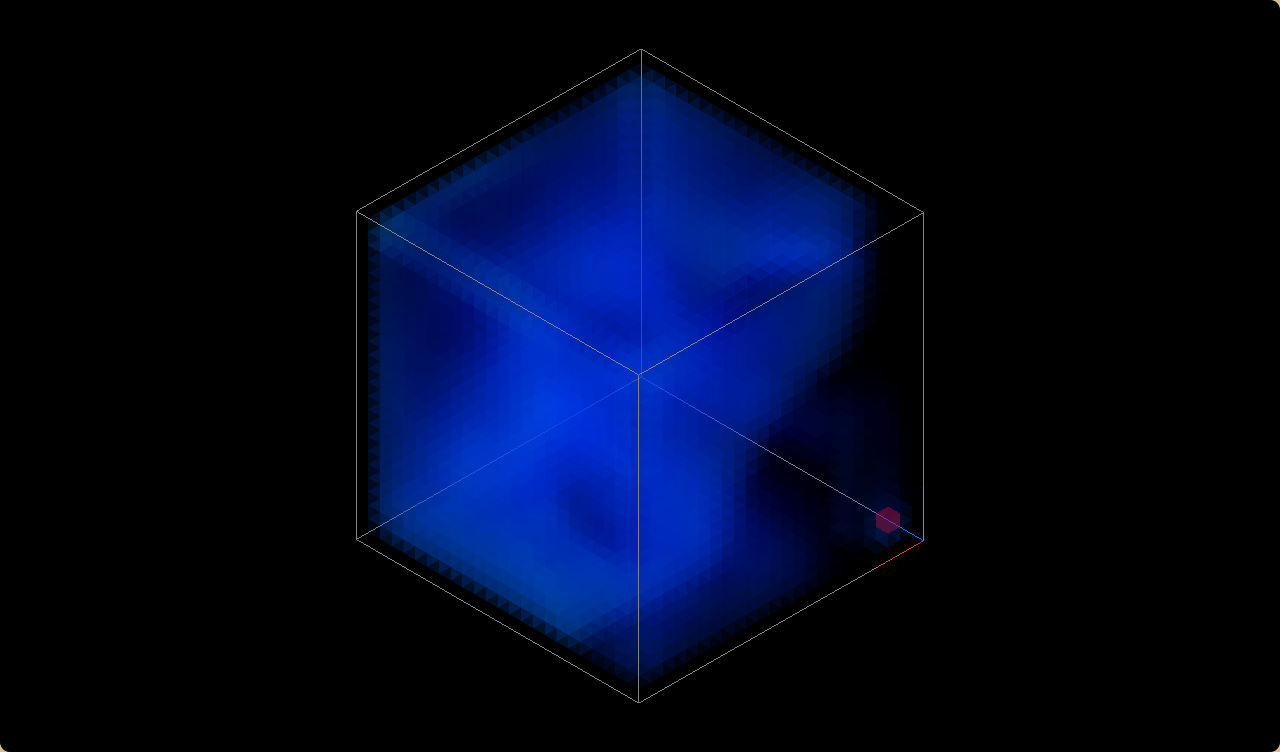
\includegraphics[height=1.65in]{resources/core2.png}
    \end{subfigure}
	\caption{Basic fluid simulation}
\end{figure}

\subsubsection{Voxelizing Geometry}
The next step is to implement geometry collision. The graphics library we're using,
Raylib, has a function to load geometry from object files. Loading in a torus is
easy enough, but the real challenge lies in communicating to the CFD that there's
a torus in a given position and it behaving correspondingly.

First, the 3D object that Raylib loads has to be converted to a BVH (Bounding Volume
Hierarchy) object. This is a tree structure that contains the object's geometry in
a way that makes it easy to check if a point is inside the object. This format
is what FCL (\href{https://github.com/flexible-collision-library/fcl}{Flexible Collision Library})
uses to check for collisions. We are using FCL to easily process flexible
collisions between 3D objects.

The next step is to write a voxelization function. Voxelization takes a 3D
object's mesh data and checks the previously established 3D vector fields to see which
if the object is in a given cell. FCL performs collision detection between two 3D objects.
In this case those two objects are our obstacle (like a torus or a plane), and
whichever cell is being iterated over. If the object is in a cell, we can pass a
condition to the CFD. This is done for every cell in the grid, and the result
is a 3D boolean array that represents the object. The source code is at \lstinline{Fluid::voxelize}.
Each obstacle is passed to this function, and as a result we get a 3D boolean
field saved at \lstinline{Fluid::state}. Below is a figure of the voxel map,
with cells classified as solid highlighted in blue.

\begin{figure}[H]
    \centering
    \begin{subfigure}[t]{0.45\textwidth}
        \centering
        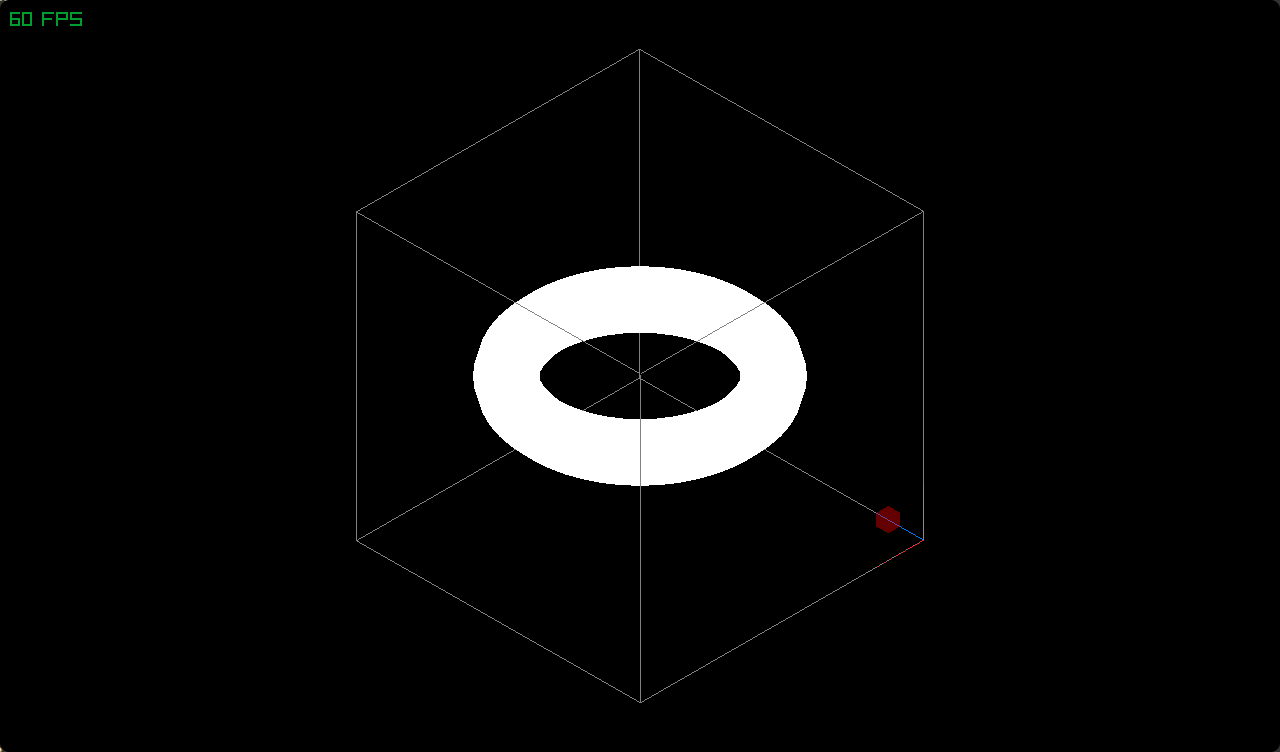
\includegraphics[height=1.65in]{resources/voxelize1.png}%
    \end{subfigure}
    \hfill
    \begin{subfigure}[t]{0.45\textwidth}
        \centering
        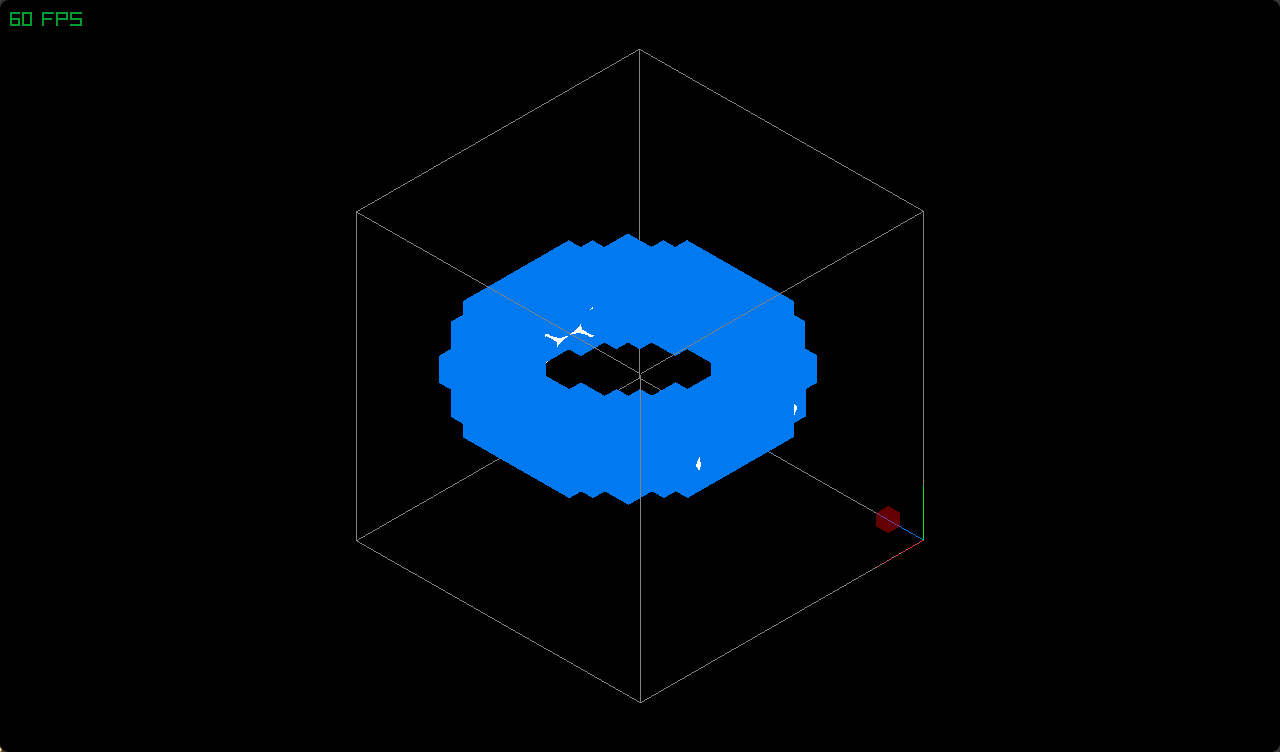
\includegraphics[height=1.65in]{resources/voxelize2.png}%
    \end{subfigure}
    \caption{Voxel map}
\end{figure}

This is called the Cut-Cell method. The reason we even need this is because
the more obvious option is to set up the grid to be high resolution so the voxels
are small enough to accurately approximate an arbitrarily complex object.
The reason this isn't viable is purely due to performance. This might be reasonable
with a supercomputer, but for our purposes we'd just like to optimize.

Another method would be to implement an AMR (Adaptive Mesh Refinement) system,
which would adapt the mesh's resolution based on what's in a given region. So this would
generate a high resolution grid around an obstacle's bounds, and a low resolution
grid in any empty space. This is an interesting concept, but we would have to
rewrite some of the fluid math code to make the irregular grid work, and it seems
like a lot of work, so we stuck with the Cut-Cell method. TODO: finish this

\subsubsection{Implementing obstacle collision}
Each cell of the grid is now one of three states: \lstinline{FLUID},
\lstinline{SOLID}, or \lstinline{CUT_CELL}. This method of classifying cells
into the three states is called the \href{https://www.sciencedirect.com/science/article/pii/S0307904X00000056}{Cut-Cell method}.
\begin{enumerate}
	\item{Fluid cells}
		\begin{itemize}
			\item{Cells that are fully inside a fluid region}
			\item{Normal Navier-Stokes equations apply}
		\end{itemize}
	\item{Solid cells}
		\begin{itemize}
			\item{Cells that are fully inside an obstacle}
			\item{Applies no-slip condition: velocity is zero}
		\end{itemize}
	\item{Cut-cells}
		\begin{itemize}
			\item{Cells partially inside an object}
			\item{Modify fluid calculations}
		\end{itemize}
\end{enumerate}

TODO: FINISH EXPLAINING CUT-CELL

TODO: EXPLAIN OUR FAILURES
TODO: EXPLAIN POSSIBLE FIXES AND WHAT SHOULD BE FINISHED/IMPROVED

% Results
\section{Results}
\ipsum[1]

% Conclusion
\subsection{Conclusion}
We our paper we tried to answer the following questions: 
\begin{itemize}
	\item{How do the different aspects of fluid dynamics work and how do we implement it in a computer program?}
	\item{How do we dynamically generate 3D models?}
	\item{How does an airplane's wing shape influence its performance?}
\end{itemize}

% References
\nocite{*}
\printbibliography

\end{document}
